\documentclass[dvipdfmx]{jsarticle}
\usepackage[dvipdfmx]{graphicx}
\usepackage{amsmath, amssymb}
\usepackage{mathtools}
\usepackage{here}
\usepackage{caption}

\renewcommand{\thefigure}{\thesection.\arabic{figure}}
\setcounter{section}{5}
\setcounter{figure}{21}

\begin{document}

\section*{5.4.1 周波数シフトキーイングと最小シフトキーイング}
MFSKでは,変調された信号は次のように与えられる.

\begin{equation}\label{}
s_i (t) = A\cos[2\pi f_c t + 2\pi \alpha_i \Delta f_c t + \phi_i], 0 \leq t < T_s
\tag{5.64}
\end{equation}

MFSK(multi frequency shift key)では,$\alpha_i = (2i - 1 - M), i = 1, 2, ..., M = 2^K$で変調信号が与えられる.
FSKキャリア間の最小周波数分離は$2\Delta f_c$となる.MFSKはM個の基底関数$\phi_i (t) = \sqrt{2/T_s} \cos [2\pi f_c t + 2\pi \alpha_i \Delta f_c t + \phi_i]$で構成され,ここで$\sqrt{2/T_s}$は$\int_0^{T_s} \phi^2 (t) = 1$を保証するための正規化係数である.あるシンボル時間において,1つの基底関数だけがチャネルを通じて伝送される.

MFSK信号を生成する簡単な方法は,図5.22に示すように,M個の発振器が異なる周波数$f_i = f_c + \alpha_i \Delta f_c$で動作し,変調器がシンボル時間$T_s$ごとにこれらの異なる発振器の間で切り替わる.
しかし,この実装では,発信器間の位相オフセットにより,スイッチング時間での位相遷移が不連続になる.

\begin{figure}[H]
\begin{center}
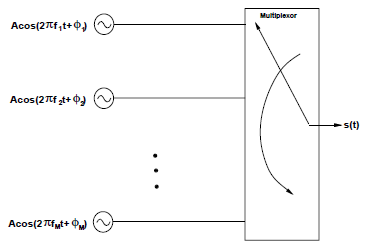
\includegraphics[width=0.6\linewidth]{./spring_lec/wc-5-4-1.png}
\end{center}
\caption{周波数変調器}
\end{figure}

\begin{figure}[H]
\begin{center}
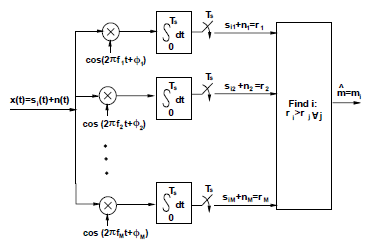
\includegraphics[width=0.6\linewidth]{./spring_lec/wc-5-4-2.png}
\end{center}
\caption{周波数復調器(コヒーレント)}
\end{figure}

\noindent
この不連続な位相は,スペクトルの広がりを招き,好ましくない.
連続した位相を維持するFSK変調器については,次節で説明する.MFSKのコヒーレント検出は,図5.4の標準的な構造を使用する.2値信号の場合は,図5.24のような構造に簡略化することができ,判定器は入力が0より大きい場合は1ビット,0より小さい場合は0ビットを出力する.

MSKはFSKの特殊なケースで,最小の周波数分離は$2\Delta f_c = 0.5/T_s$です.復調には信号の直交性が必要なので,$2\Delta f_c = 0.5/T_s$はFSKで可能な最小の周波数分離であり,したがって最小の帯域幅を占有することに注意しなくてはならない.

\begin{figure}[H]
\begin{center}
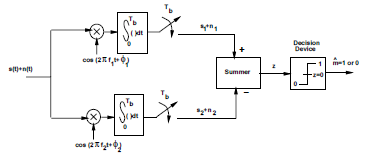
\includegraphics[width=0.6\linewidth]{./spring_lec/wc5-4-3..png}
\end{center}
\caption{FSK用復調器}
\end{figure}

\begin{figure}[H]
\begin{center}
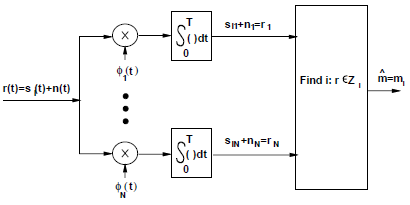
\includegraphics[width=0.6\linewidth]{./spring_lec/wc5-4-0.png}
\end{center}
\caption*{図5.4: AWGNにおける信号検出のための受信機構造}
\end{figure}
\end{document}